\chapter{Informations- und Technologierecht}

\section{Datenbearbeitung im Internet}
\subsection{Begriffe}
\begin{description}
  \item[Datenschutz] Schutz der Persönlichkeit und der Grundrechte der Person, über die Daten bearbeitet werden. Teil des Persönlichkeitsrechtes.
  \item[Personendaten] Alle Angaben, die sich auf eine bestimmte oder \textit{bestimmbare} Person beziehen. Bsp: Adresse, Vor-/Nachname, Geburtsdatum etc.  
  \item[Datenbearbeitung] ist ein Eingriff in die Persönlichkeitsrechte. Ohne Rechtfertigung dazu ist der Eingriff \textit{widerrechtlich}. Mögliche Rechtfertigungsgründe: Einwilligung der betroffenen Person, überwiegendes privates oder öffentliches Interesse, beispielsweise Recherche über potenzielle Vertragspartner.. aber immer im Ermessen, oder gesetzliche Grundlage.
  \item[Rechte der betroffenen Person] Auskunftsrecht, Sperr-, Korrektur und Löschungsrecht (DSG) Persönlichkeitsverletzung, Schadenersatz/Genugtuung (Zivilrecht) Unbefugte Datenbeschaffung, unbefugtes Eindringen in oder betrügerischer Missbrauch einee Datenverarbeitungsanlage, Datenbeschädigung (Strafrecht)
  \item[Privacy Policy] Datenbearbeitungserklärung. Orientiert darüber, nach welchem selbst auferlegten Prinzipien ein Unternehmen Personendaten (insbesondere von Kunden) bearbeitet. Kann vom Kunden vollständig oder teilweise akzeptiert werden. Anforderungen:
    \begin{itemize}
      \item Auffindbar: Konvention im Web auf der Startseite ganz Unten
      \item Welche Daten werden zu welchen Zwecken erhoben
      \item ... an Dritte weitergegeben?
      \item Wie lange werden Daten aufbewahrt?
      \item Stehen dem Benutzer Wahlmöglichkeiten zur Bearbeitung seiner Daten zu?
      \item Welche Rechte hat der Benutzer? Auskunfts-, Berichtigungsrecht, ...
      \item Welche Stelle beantwortet Fragen über die Bearbeitung der Daten?
      \item Welche Sicherheitsmassnahmen werden zum Schutz von Personendaten angewendet?
      \item Werden Cookies oder Analyse- / Tracking-Tools verwendet?
    \end{itemize}
\end{description}

\begin{figure}[H]
  \centering
  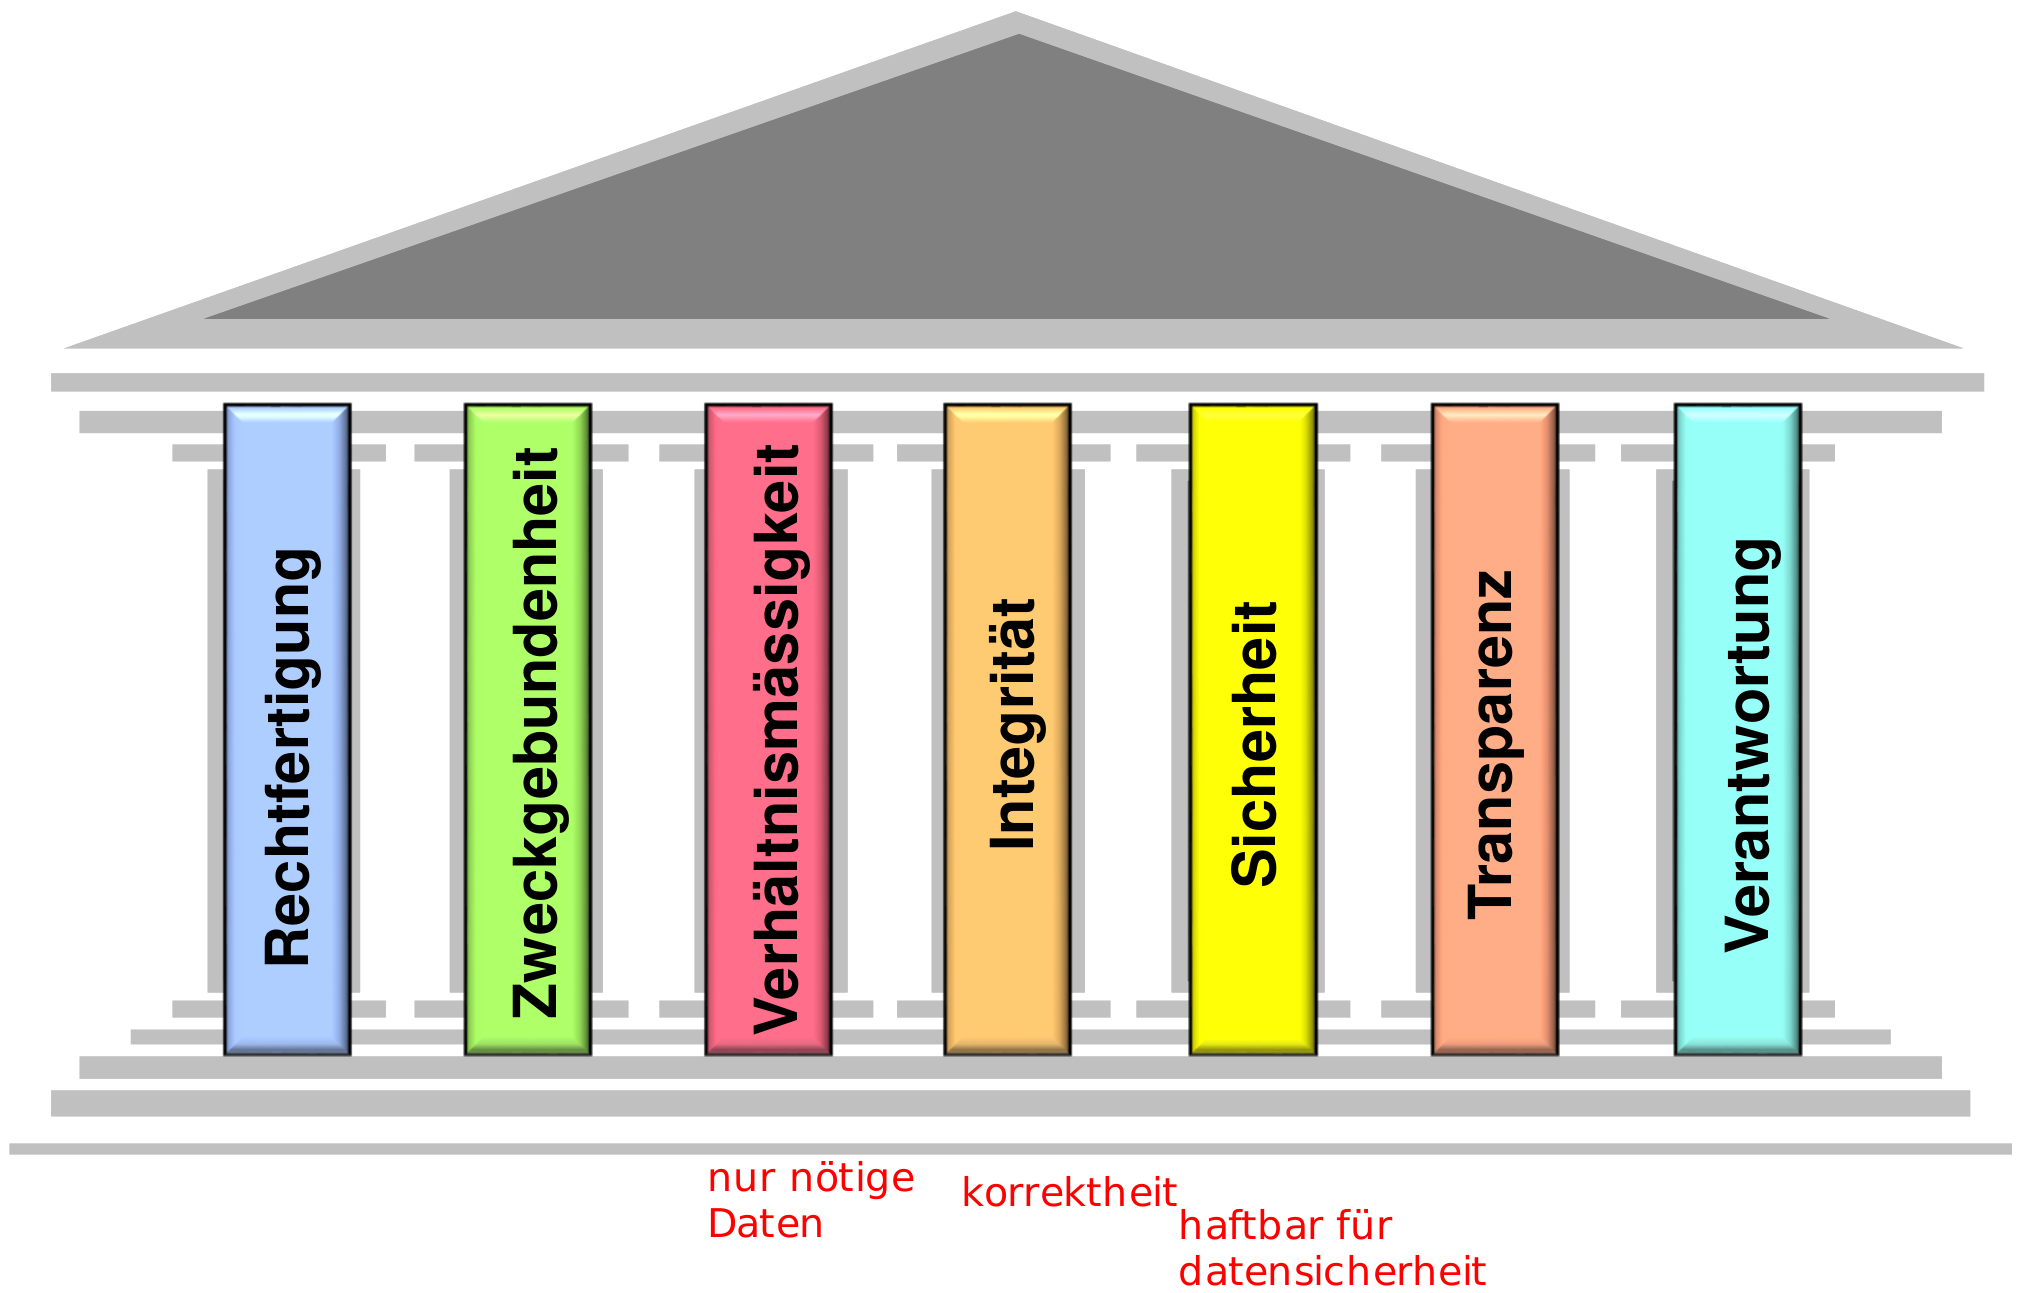
\includegraphics[width=10cm]{res/datenschutz-grundprinzipien.png}
  \caption{Datenschutzrechtliche Grundprinzipien}
\end{figure}

\subsection{Datenschutzgesetze}

\begin{description}
  \item[Bund:] Bundesgesetz über den Datenschutz (DSG). Geltungsbereich: Privatpersonen und private Unternehmungen, Bundesorgane.
  \item[Kantone:] Eigene Datenschutzgesetze, z.B. DSG SG. Geltungsbereich: öffentliche Organe auf kantonaler und kommunaler Ebene, mit öffentlichen Aufgaben betraute Private 
\end{description}

\subsection{Kundenbindungsprogramme}

Marketinginstrument zur Gewinnung \textbf{künftiger}, \textbf{aktueller} und \textbf{ehemaliger} Kunden. 
Anreize für wiederholte Geschäftsbeziehungen in Form von \textbf{Prämien}, \textbf{Rabatten} etc.
Verwendung von Kundendaten für die Erstellung von \textbf{Kundenprofilen} und \textbf{Direktmarketing}, Bonus- und Punkteprogramme.

\begin{figure}[H]
  \centering
  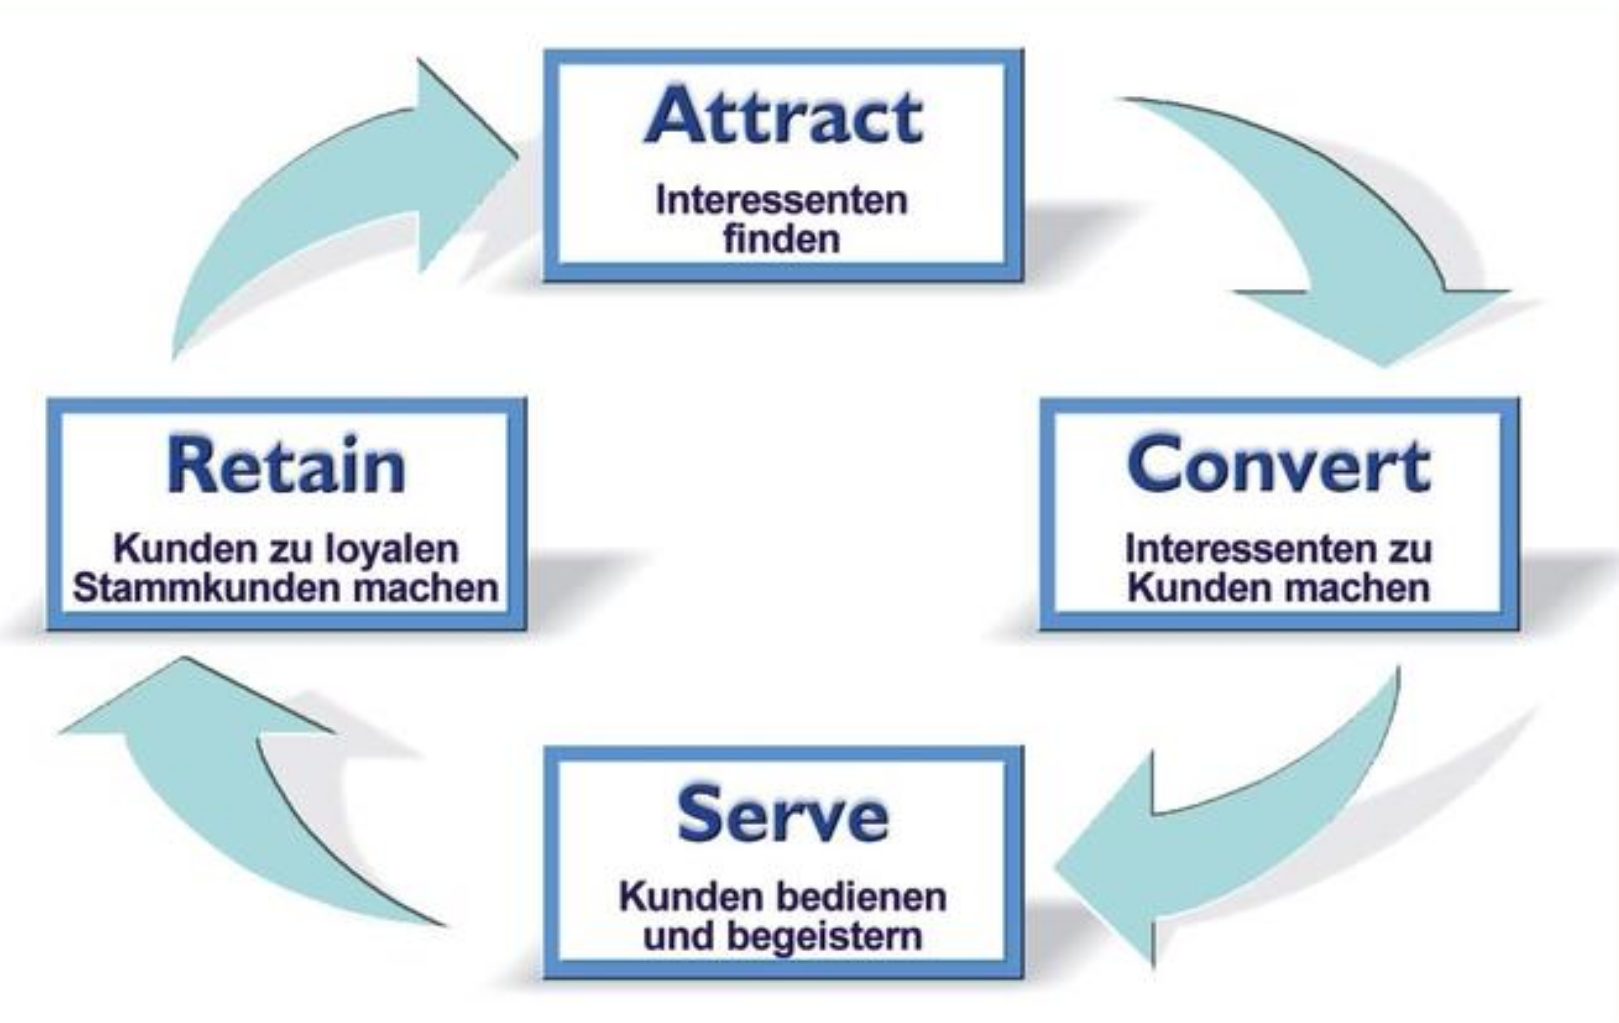
\includegraphics[width=8cm]{res/kundenbindung-kreislsauf.png}
  \caption{Kreislauf Kundenbindungsprogramm}
\end{figure}

\subsubsection*{Personalisierung im Onlinemarketing}
\begin{description}
  \item[Personal Pricing:] Angebot / Preis richtet sich nach der Kaufkraft des Käufers. Beispiel: Flugtickets. Mittel: Geolocation, Hardware (besitzt ein teures Notebook). Soll bald nicht mehr legal sein.
  \item[Kollaboratives Filtern:] Empfehlungen gestützt auf Nutzungsverhalten anderer Nutzer. Beispiel: Amazon, Netflix.
  \item[Technologien:] Data-Mining, Filtertechnologien, Cookies, Beacon, Augmented Reality   
\end{description}

\subsection{Anmeldung Datensammlung}
\textbf{Art. 11a DSG} verpflichtet Privatpersonen zur Anmeldung von Datensammlung beim \textit{Eidgenössischen Datenschutz- und Öffentlichkeitsbeauftragten EDÖB}, falls:
\begin{itemize}
  \item regelmässig besonders schützenswerte Personendaten oder Persönlichkeitsprofile bearbeitet werden \textit{oder}
  \item regelmässig Personendaten an Dritte bekannt gegeben werden.
\end{itemize}

\noindent
Ausnahmen: Art. 11a Abs. 5 DSG: 
  \textit{Entgegen den Bestimmungen der Absätze 2 und 3 muss der Inhaber von Datensammlungen seine Sammlungen nicht anmelden, wenn:}

\textit{a. private Personen Daten aufgrund einer gesetzlichen Verpflichtung bearbeiten;}

\textit{b. der Bundesrat eine Bearbeitung von der Anmeldepflicht ausgenommen hat, weil sie die Rechte der betroffenen Personen nicht gefährdet;}

\textit{c. er die Daten ausschliesslich für die Veröffentlichung im redaktionellen Teil eines periodisch erscheinenden Mediums verwendet und keine Daten an Dritte weitergibt, ohne dass die betroffenen Personen davon Kenntnis haben;}

\textit{d. die Daten durch Journalisten bearbeitet werden, denen die Datensammlung ausschliesslich als persönliches Arbeitsinstrument dient;}

\textit{e. er einen Datenschutzverantwortlichen bezeichnet hat, der unabhängig die betriebsinterne Einhaltung der Datenschutzvorschriften überwacht und ein Verzeichnis der Datensammlungen führt;}

\textit{f. er aufgrund eines Zertifizierungsverfahrens nach Artikel 11 ein Datenschutz-Qualitätszeichen erworben hat und das Ergebnis der Bewertung dem Beauftragten mitgeteilt wurde.}

\subsection{Datensicherheit}
\textit{CIA}: Vertraulichkeit, Verfügbarkeit, Integrität müssen durch organisatorische und technische Massnahmen sichergestellt werden.

\subsection{Grenzüberschreitende Bekanntgabe von Daten}
\textbf{Art. 6 DSG} verlangt angemessenen Schutz von ins Ausland übermittelten Daten durch
\begin{itemize}
  \item genügende Gesetzgebung im Zielland
  \item \textbf{oder} hinreichende vertragliche Garantien des Empfängers bzw. Verschlüsselung oder Pseudonymisierung / Anonymisierung
\end{itemize}

Beispiel EU: gleichwertiges Datenschutzniveau. Keine Aktion nötig. USA: kein gleichwertiges Datenschutzniveau, DSG nur in einzelnen Bundesstaaten vorhanden. Vorgabe von \textbf{Standard Contractual Clauses} der Schweiz möglich bzw. nötig.

Angemessener Schutz nach EDÖB Liste:
Andorra, Belgien, Bulgarien, Dänemark, Deutschland, Estland, Färöer, Finnland, Frankreich, Gibraltar, Griechenland, Guernsey, Irland, Island, Isle of Man, Italien, Jersey, Kroatien, Lettland, Liechtenstein, Litauen, Luxemburg, Malta, Monaco, Niederlande, Norwegen, Österreich, Polen, Portugal, Rumänien, Schweden, Slowakei, Slowenien, Spanien, Tschechien, Ungarn, UK, Zypern || Kanada, Argentinien, Uruguay, Israel, Neuseeland. Schutz unter bestimmten Voraussetzungen: Australien.

\section{E-Commerce}

\subsection{Voraussetzungen zum Zustandekommen eines Vertrags}

Parteien sind handlungsfähig, also volljährig und urteilsfähig.
Konsens: übereinstimmende gegenseitige Willensäusserung.
  
\noindent
  \textbf{OR 1} 
  
  \textit{
    1 Zum Abschlusse eines Vertrages ist die übereinstimmende gegenseitige Willensäusserung der Parteien erforderlich.}
    
  \textit{2 Sie kann eine ausdrückliche oder stillschweigende sein.}

\vspace{3mm}
\noindent
Alle objektiv und subjektiv wesentlichen Vertragspunkte sind geklärt.
    
\noindent
  \textbf{OR 2} 
    
  \textit{
    1 Haben sich die Parteien über alle wesentlichen Punkte geeinigt, so wird vermutet, dass der Vorbehalt von Nebenpunkten die Verbindlichkeit des Vertrages nicht hindern solle.}
    
  \textit{
    2 Kommt über die vorbehaltenen Nebenpunkte eine Vereinbarung nicht zustande, so hat der Richter über diese nach der Natur des Geschäftes zu entscheiden.}
      
  \textit{
    3 Vorbehalten bleiben die Bestimmungen über die Form der Verträge.}

\vspace{3mm}
\noindent
Antrag und Annahme führt zum Vertragsschluss.
  
\noindent
  \textbf{OR 3} 
  
  \textit{
    1 Wer einem andern den Antrag zum Abschlusse eines Vertrages stellt und für die Annahme eine Frist setzt, bleibt bis zu deren Ablauf an den Antrag gebunden.}
  
  \textit{
    2 Er wird wieder frei, wenn eine Annahmeerklärung nicht vor Ablauf dieser Frist bei ihm eingetroffen ist.}

\subsection{Vertragsabschluss im Internet}

Grundsätzlich formlos gültig, falls schriftlich dann kann eine digitale Signatur angewendet werden.

\noindent
\textbf{OR 11}

  \textit{
  1 Verträge bedürfen zu ihrer Gültigkeit nur dann einer besonderen Form, wenn das Gesetz eine solche vorschreibt.}

  \textit{2 Ist über Bedeutung und Wirkung einer gesetzlich vorgeschriebenen Form nicht etwas anderes bestimmt, so hängt von deren Beobachtung die Gültigkeit des Vertrages ab.}

  \noindent
  \textbf{OR 14} 

  \textit{1 Die Unterschrift ist eigenhändig zu schreiben.}

  \textit{2bis Der eigenhändigen Unterschrift gleichgestellt ist die mit einem qualifizierten Zeitstempel verbundene qualifizierte elektronische Signatur gemäss Bundesgesetz vom 18. März 2016 über die elektronische Signatur. \ldots}
  \vspace{3mm}

In der Regel stellt ein Internet-Angebot eine unverbindliche Einladung zur Antragsstellung dar. Bestätigung des Verkäufers nötig, um Vertrag abzuschliessen. Ausnahme: Internet-Auktion, Download von Programmen etc.

\noindent
\textbf{OR 7}

\textit{2 Die Versendung von Tarifen, Preislisten u. dgl. bedeutet an sich keinen Antrag.}
\vspace{3mm}

Vertragsschluss unter Abwesenden, bedeutet keine unmittelbare Reaktion auf die Willenserklärung. Entscheidung des Adressaten über die Annahme des Angebotes soll "innert angemessener Frist" geschehen.

\noindent
\textbf{OR 5}

\textit{1 Wird der Antrag ohne Bestimmung einer Frist an einen Abwesenden gestellt, so bleibt der Antragsteller bis zu dem Zeitpunkte gebunden, wo er den Eingang der Antwort bei ihrer ordnungsmässigen und rechtzeitigen Absendung erwarten darf.}

\textit{2 Er darf dabei voraussetzen, dass sein Antrag rechtzeitig angekommen sei.}

\textit{3 Trifft die rechtzeitig abgesandte Annahmeerklärung erst nach jenem Zeitpunkte bei dem Antragsteller ein, so ist dieser, wenn er nicht gebunden sein will, verpflichtet, ohne Verzug hievon Anzeige zu machen.}

\subsection{Folgen eines Vertragsschlusses}
Die Folgen eines Vertragsschlusses ist die Begründung von Rechten und Pflichten (Forderungen) beiderseits. 

\subsection{AGB: Allgemeine Geschäftsbedingungen}

AGB beschreiben für eine Vielzahl von Verträgen vorformulierte Bedingungen. Sie können abweichende oder ergänzende Regelungen zum Gesetz beinhalten. Sind in der Schweiz nur teilweise gesetzlich geregelt. Ziel: Vereinfachung, Beschleunigung und Standardisierung von Verträgen.

\noindent
Zur Vertragsfreiheit, Inhaltsfreiheit:

\noindent
\textbf{OR 19}

\textit{1 Der Inhalt des Vertrages kann innerhalb der Schranken des Gesetzes beliebig festgestellt werden.}

\begin{description}
  \item[Verbindlichkeit] 
  Sind Vertragsbestandteil. Möglichkeit der Kenntnisnahme, müssen verständlich und lesbar sein. Zustimmung kann ausdrücklich oder stillschweigend sein: Teil des Vertrags, deutlicher Hinweis.

  \item[Branchenspezifische AGB]
  In manchen Branchen gibt es vorgefertigte Normen, bsp. SIA für Bauarbeiten.

  \item[Inhalt]
  Mögliche Punkte sind der Zeitpunkt des Vertragsabschlusses, Widerrufsmöglichkeit, Zahlungsbedingungen, Lieferbedingungen, Gewährleistung, Garantie, Haftung, Gerichtsstand, anwendbares Recht, etc.

  \item[Gefahren]
  Zustimmung geschieht häufig ohne Kenntnisnahme von deren Inhalt. einseitige Verteilung von Rechten und Pflichten zugunsten der Partei, die die AGB schreibt. Bsp: Wegbedingung der Haftung, Verrechnungsverzicht etc.
  Unklare oder ungewöhnliche Regelungen.
  Sog. 'Take it or leave it' Contracts entstehen, wenn ganze Wirtschaftszweige ihre AGB untereinander absprechen.

  \item[Grenzen]
  Abweichende Individualabreden haben Vorrang. Beachtet werden müssen zwingendes Recht, gute Sitten, Persönlichkeitsrecht

  \textbf{OR 19}

  \textit{2 Von den gesetzlichen Vorschriften abweichende Vereinbarungen sind nur zulässig, wo das Gesetz nicht eine unabänderliche Vorschrift aufstellt oder die Abweichung nicht einen Verstoss gegen die öffentliche Ordnung, gegen die guten Sitten oder gegen das Recht der Persönlichkeit in sich schliesst.}

  Verwendung missbräuchlicher Geschäftsbedingungen
  
  \textbf{UWG 8}

  \textit{Unlauter handelt insbesondere, wer allgemeine Geschäftsbedingungen verwendet, die in Treu und Glauben verletzender Weise zum Nachteil der Konsumentinnen und Konsumenten ein erhebliches und ungerechtfertigtes Missverhältnis zwischen den vertraglichen Rechten und den vertraglichen Pflichten vorsehen.}

  \item[Auslegung] Grundsätzlich gelten Willens- und Vertrauensprinzip wie bei individuell verfassten Abreden. Unklare Bestimmungen werden im Zweifelsfalle zu\textit{un}gunsten des Verfassers ausgelegt (Unklarheitenregel). AGB, mit deren Inhalten der Zustimmende nicht rechnen muss, gelten nicht (Ungewöhnlichkeitsregel). Ausnahme hierzu: besodere Hervorhebung (optisch), Zustimmender hat Kenntnis vom Inhalt ("Vollübernahme"), ist geschäfts- und branchenerfahren, Bestimmung enthält keinen objektiv geschäftsfremden Inhalt.
\end{description}

\subsection{Internationale Verhältnisse}

Problematik bei immer mehr zunehmenden internationalen Geschäftsbeziehungen, Bestellungen bei Shops im Ausland:
Recht ist national auf das Staatsgebiet beschränkt. Verschiedene Rechtsordnungen können einander widersprechen. International vereinheitlichtes Recht besteht nur beschränkt.

\begin{description}
  \item[Kollisionsrecht] Als "Rückfallebene" gilt das Bundesgesetz über das Internationale Privatrecht, bilaterale oder multilaterale Staatsverträge haben stets Vorrang, wenn vorhanden. 
  \item[LugÜ 2007:]
  \textit{
    Das Übereinkommen über die gerichtliche Zuständigkeit und die Anerkennung und Vollstreckung von Entscheidungen in Zivil- und Handelssachen (Lugano-Übereinkommen, LugÜ) ist am 30. Oktober 2007 in Lugano geschlossen worden. Unterzeichner sind die Schweizerische Eidgenossenschaft, die Europäische Gemeinschaft, das Königreich Dänemark, das Königreich Norwegen und die Republik Island.}
    \item[EU: Verordnung zu vertraglichen Schuldverhältnissen]
    \item[EU: Richtlinie zu vertraglichen Aspekten des Warenkaufs]
    \item[EU: Richtlinie über den elektronischen Geschäftsverkehr] gilt für Konsumenten mit Wohnsitz in der EU und dem EWR. Statuiert Informationspflicht für Anbieter: Angaben über Produkt, Preis (inkl. aller Abgaben), Lieferung, Angaben über Anbieter wie Firma, Sitz, Kontaktdaten, MwSt. Nummer, unverzügliche elektronische Bestätigung des Vertagsabschlusses. Konsument verfügt automatisch über ein \textbf{Widerrufsrecht}
  \end{description}
    
\section{Cybercrime und Spam}

\begin{description}
  \item[Merkmale Cybercrime] Folge der rasanten Entwicklung der Informations- und Netzwerktechnik in den letzten 20-30 Jahren, bedeutet starke Zunahme der Cyberkriminalität, transnationaler Kriminalität. Grosser wirtschaftlicher Schaden.
  \item[Formen] Phishing, Spyware/Ransomware, DDoS Angriff, Identitätsdiebstahl, Romance Scam / Sextorsion, Darknet als online Schwarzmarkt, etc.
  \item[Abkommen / Stellen] Übereinkommen über die Cyberkriminalität (global), Europaratsübereinkommen über die Cyberkriminalität (EU), MELANI / KOBIK / NCSC (Schweizer Bund), Kompentenzzentren Cybercrime (Kantonal)
  \item[Strafbarkeit in der Schweiz] Angelehnt an traditionelle Strafnormen sind 1995 neue Straftatbestände geschaffen worden. Diebstahl / Datendiebstahl, Betrug / Computerbetrug,  Sachbeschädigung / Datenbeschädigung. Strafverfolgung bisher noch eher zurückhhaltend.
\end{description}

\subsection{Allgemeine Strafbarkeit}

Allgemeine Strafbarkeitsvoraussetzungen: Tatbestandsmässigkeit (objektiv und subjektiv), Rechtswidrigkeit (keine Rechtfertigungsgründe vorhanden), Schuld (keine Schuldausschlussgründe vorhanden)

Objektiver Tatbestand: Verstoss gegen gesetzliche Bestimmungen

Subjektiver Tatbestand: Vorsatz zum Schaden
\vspace{3mm}

\subsection{Computerdelikte}

\textbf{StGB 143 - unbefugte Datenbeschaffung}

\textit{1 Wer in der Absicht, sich oder einen andern unrechtmässig zu bereichern, sich oder einem andern elektronisch oder in vergleichbarer Weise gespeicherte oder übermittelte Daten beschafft, die nicht für ihn bestimmt und gegen seinen unbefugten Zugriff besonders gesichert sind, wird mit Freiheitsstrafe bis zu fünf Jahren oder Geldstrafe bestraft.}

\textit{2 Die unbefugte Datenbeschaffung zum Nachteil eines Angehörigen oder Familiengenossen wird nur auf Antrag verfolgt.}
\vspace{3mm}

\noindent
\textbf{StGB 143bis - unbefugtes Eindringen in ein Datenverarbeitungssystem}

\textit{1 Wer auf dem Wege von Datenübertragungseinrichtungen unbefugterweise in ein fremdes, gegen seinen Zugriff besonders gesichertes Datenverarbeitungssystem eindringt, wird, auf Antrag, mit Freiheitsstrafe bis zu drei Jahren oder Geldstrafe bestraft.}

\textit{2 Wer Passwörter, Programme oder andere Daten, von denen er weiss oder annehmen muss, dass sie zur Begehung einer strafbaren Handlung gemäss Absatz 1 verwendet werden sollen, in Verkehr bringt oder zugänglich macht, wird mit Freiheitsstrafe bis zu drei Jahren oder Geldstrafe bestraft.}
\vspace{3mm}

\noindent
\textbf{StGB 144bis - Datenbeschädigung}

Malware, Schadprogramme die vom Benutzer unerwünschte, meist schädliche Funktionen ausführen. Computervirus, Computerwurm, Trojaner, Spyware, \ldots

\textit{1 Wer unbefugt elektronisch oder in vergleichbarer Weise gespeicherte oder übermittelte Daten verändert, löscht oder unbrauchbar macht, wird, auf Antrag, mit Freiheitsstrafe bis zu drei Jahren oder Geldstrafe bestraft. 
Hat der Täter einen grossen Schaden verursacht, so kann auf Freiheitsstrafe von einem Jahr bis zu fünf Jahren erkannt werden. Die Tat wird von Amtes wegen verfolgt.}

\textit{2 Wer Programme, von denen er weiss oder annehmen muss, dass sie zu den in Ziffer 1 genannten Zwecken verwendet werden sollen, herstellt, einführt, in Verkehr bringt, anpreist, anbietet oder sonst wie zugänglich macht oder zu ihrer Herstellung Anleitung gibt, wird mit Freiheitsstrafe bis zu drei Jahren oder Geldstrafe bestraft.
Handelt der Täter gewerbsmässig, so kann auf Freiheitsstrafe von einem Jahr bis zu fünf Jahren erkannt werden.}
\vspace{3mm}

\noindent
\textbf{StGB 147 - betrügerischer Missbrauch einer Datenverarbeitungsanlage}

\textit{1 Wer in der Absicht, sich oder einen andern unrechtmässig zu bereichern, durch unrichtige, unvollständige oder unbefugte Verwendung von Daten oder in vergleichbarer Weise auf einen elektronischen oder vergleichbaren Datenverarbeitungs- oder Datenübermittlungsvorgang einwirkt und dadurch eine Vermögensverschiebung zum Schaden eines andern herbeiführt oder eine Vermögensverschiebung unmittelbar darnach verdeckt, wird mit Freiheitsstrafe bis zu fünf Jahren oder Geldstrafe bestraft.}

\textit{2 Handelt der Täter gewerbsmässig, so wird er mit Freiheitsstrafe bis zu zehn Jahren oder Geldstrafe nicht unter 90 Tagessätzen bestraft.}

\textit{3 Der betrügerische Missbrauch einer Datenverarbeitungsanlage zum Nachteil eines Angehörigen oder Familiengenossen wird nur auf Antrag verfolgt.
}

\subsubsection{Überwachung des Post- und Fernmeldeverkehrs (ÜPF)}

Auswertung des Post- und Fernmeldeverkehrs zur Klärung von schweren Straftaten
Auf Anordnung durch Staatsanwaltschaft, Genehmigung durch Zwangsmassnahmengericht.

Der Dienst ÜPF ist der unabhängige Dienst für die Überwachung des Post- und Fernmeldeverkehrs in der Schweiz. Er wacht über die rechtskonforme, rechtsstaatliche Umsetzung von Überwachungen des Post- und Fernmeldeverkehrs zum Schutze der Privatsphäre der Bevölkerung. Im Weiteren stellt er sicher, dass im Bereich der strafprozessualen Überwachung des Post- und Fernmeldeverkehrs die geltenden Vorgaben eingehalten werden.

\subsubsection{Was tun im Schadenfall}
\begin{description}
  \item[Schadenersatz aus unerlaubter Handlung: OR 4]

  \textit{1 Wer einem andern widerrechtlich Schaden zufügt, sei es mit Absicht, sei es aus Fahrlässigkeit, wird ihm zum Ersatze verpflichtet.}
  
  \textit{2 Ebenso ist zum Ersatze verpflichtet, wer einem andern in einer gegen die guten Sitten verstossenden Weise absichtlich Schaden zufügt.}
  \vspace{3mm}
  
  \item[Schadenersatz aus Vertrag: OR 97]

  \textit{1 Kann die Erfüllung der Verbindlichkeit überhaupt nicht oder nicht gehörig bewirkt werden, so hat der Schuldner für den daraus entstehenden Schaden Ersatz zu leisten, sofern er nicht beweist, dass ihm keinerlei Verschulden zur Last falle.}

  \textit{2 Für die Vollstreckung gelten die Bestimmungen des Bundesgesetzes vom 11. April 188943 über Schuldbetreibung und Konkurs sowie der Zivilprozessordnung vom 19. Dezember 200844 (ZPO).45}
  \item[Cyberversicherung] Mögliche Versicherung für Schäden aus Cyberkriminalität. Haftung für Eigen- und Drittschäden (Kostenübernahme für Betriebsunterbruch, Datenwieder-
herstellung, Krisenmanagement, Rechtsschutz etc.) Probleme: teils extensive Haftungsausschlüsse.
  \item[Schutzmassnahmen] Antivirus / Firewall einschalten, regelmässige Updates, Notfallplan und Backups, Wahl des "richtigen" OS und Browser, vorsichtiges Verhalten bei unbekannten Links, Dateien, ev. Beizug externer IT Forensiker in Notfällen.
\end{description}

\subsection{Spam}
Unerwünschte, auf elektronischem Weg übertragene Nachrichten, z.B. Massen-Emails. Häufig werbender Inhalt.

\begin{description}
  \item[Auswirkungen] Grosse Schäden in der weltweiten Kommunikation: Verlangsamung und Behinderung des legalen Datenverkehrs, grosser Aufwand zur Bearbeitung zusätzlicher überflüssiger Datenmenge.
  \item[Unlauterer Wettbewerb] wenn nicht vorher die Einwilligung des Kunden eingeholt wird (Newsletter opt-in), der Absender korrekt angegeben wird und der Kunde problem- und kostenlos die weitere Zustellung ablehnen kann. Ausnahme, 
  \item[USG 3 Bst. o] \textit{Unlauter handelt, wer Massenwerbung ohne direkten Zusammenhang mit einem angeforderten Inhalt fernmeldetechnisch sendet oder solche Sendungen veranlasst und es dabei unterlässt, vorher die Einwilligung der Kunden einzuholen, den korrekten Absender anzugeben oder auf eine problemlose und kostenlose Ablehnungsmöglichkeit hinzuweisen; wer beim Verkauf von Waren, Werken oder Leistungen Kontaktinformationen von Kunden erhält und dabei auf die Ablehnungsmöglichkeit hinweist, handelt nicht unlauter, wenn er diesen Kunden ohne deren Einwilligung Massenwerbung für eigene ähnliche Waren, Werke oder Leistungen sendet.}
  \item[Anbieter von Fernmeldediensten (Provider)] 
  
  müssen ihre Kunden vor dem Erhalt unlauterer Massen  werbung schützen

  dürfen unlautere Massenwerbung unterdrücken

  müssen den Versand unlauterer Massenwerbung durch ihre Kunden sperren bzw. den Aufbau entsprechender Verbindungen über ihre Fernmeldenetze verhindern

  dürfen unlautere Massenwerbung versendende oder weiterleitende Kunden vom Fernmeldenetz trennen
  
  müssen eine Meldestelle für den Versand unlauterer Massenwerbung über ihre Fernmeldenetze betreiben
\end{description}
